\subsection{Circadian entrainment phase: Towards a unified mathematical
model}

The perfect coordination of the oscillation periods between a
circadian system and its environment is not the only phenomenon in
chronobiology. Those periods can be perfectly aligned, but the
relative phase of this alignment, or the entrainment phase, is a not
less important feature of circadian entrainment and has been focus of
research for many decades, see, for
instance,~\cite{pittendrigh1981circadian}. Within this project, we
attempted to describe the behaviour of the entrainment phase in as
simple a mathematical model as possible and to uncover some common
patterns of its reaction to changes in the environment.

\subsubsection{Human chronotypes and the 180 degree rule}
A first striking example of the apparent unpredictability of
entrainment phase is the discrepancy between how precise our clocks
are in terms of the internal period and how broadly distributed are
our wake-up times. The reported precision of the clock is within a
quarter of hour, whereas the wake-up times (as a proxy of entrainment
phase) has a characteristic deviation of two hours across human
population \cite{duffy2005entrainment}. If our clocks are so precise,
why are our alarms not so?

We presented an attempt of clarification of this disproportion between
the precision of period and entrainment phase by introducing the
so-called 180-degree rule~\cite{granada2013human}. The rule asserts
that within a population with a however broad or narrow distribution
of internal periods $\tau$, corresponding distributions of phases
of entrainment as broad as 180 degrees are inevitable. Moreover, the
width of the entrainment range of the subject determines the
sensitivity of the entrainment phase to the mismatch between the
Zeitgeber period $T$ (usually close to 24 hours) and the internal
period $\tau$.

The explanation for the 180 degree rule is based on the inspection of
the structure of entrainment range in the simplest mathematical
oscillator models.  The phase of entrainment assumes maximal and
minimal values at the borders of entrainment range and the those
values span an interval of 180 degrees. Now if the oscillator is
easily entrainable (or ``weak'' as we call it), it has a wide
entrainment range in terms of tolerated mismatches between $\tau$ and
$T$ and, consequently, small changes in $\tau-T$ (by changing $\tau$
for example across the population) are translated into relatively
small changes of entrainment phase. If, on the other hand, the
oscillator is ``strong'', i.e. it entrainment range is narrow in terms
of $\tau-T$, small changes in $\tau$ would be translated in large
changes of entrainment phase. Given the precision of circadian rhythms
in mammals, including humans, it is thus of no surprise that a narrow
distribution of $\tau$ across the population causes a broad
distribution of entrainment phases aka wake-up times.

\begin{figure}
\begin{center}
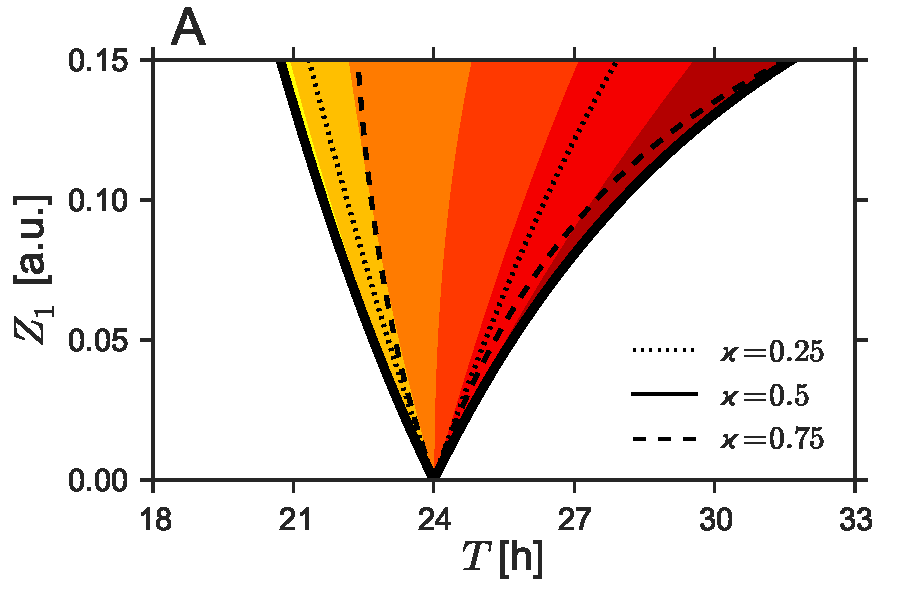
\includegraphics[width=0.49\linewidth]{figures/phase/fig1A.pdf}
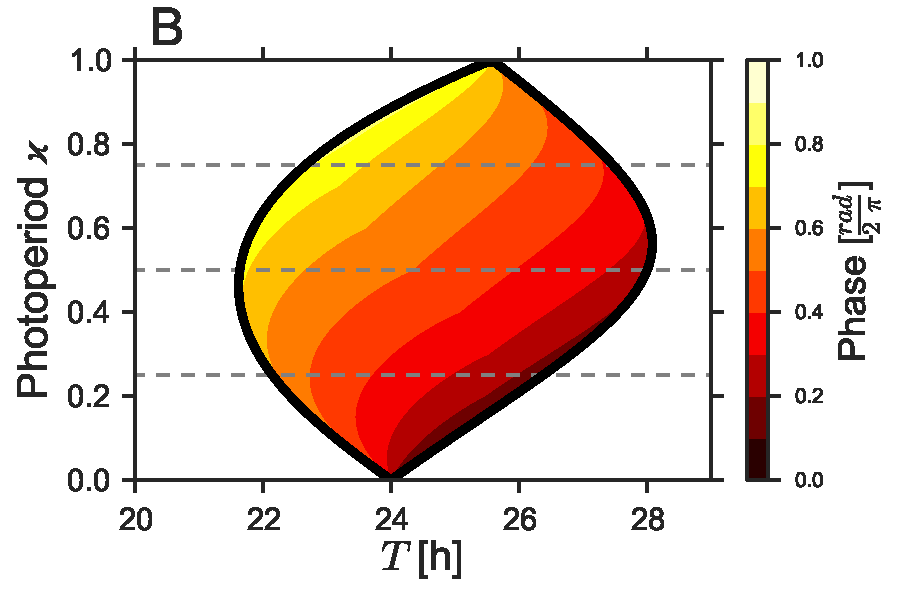
\includegraphics[width=0.49\linewidth]{figures/phase/fig1B.pdf}
\end{center}
\caption{
  {\bf A} Dependence of phase of entrainment within an Arnold tongue
  on Zeitgeber period $T$ and strength $Z_1$ for different
  photoperiods $\chi$.
  {\bf B} Dependence of phase of entrainment within an onion-like
  region on Zeitgeber period $T$ and photoperiod $\chi$.
\label{fig::phase}
}
\end{figure}

\subsubsection{Phase of entrainment in seasonality}
The phase of entrainment has been shown to be affected by the mismatch
between the internal clock period $\tau$ and the Zeitgeber period $T$.
Additionally, it is quite intuitive that a stronger Zeitgeber can
enforce its period $T$ on the internal clock even if the mismatch
between $\tau$ and $T$ is relatively large. Those facts results in
what is known as the Arnold tongue - a wedge-shaped entrainment
region, exemplarily shown in Figure~\ref{fig::phase} (A) with colours
encoding the phase of entrainment. We indeed see that the maximal
(yellowish) and the minimal (deep red) values of entrainment phases
are achieved close to the borders of the tongue.

But what if instead of changing Zeitgeber strength directly, we
consider changing photoperiod (the proportion of the light and dark
portion of the day) throughout the seasons? Intuitively we might
assume that a 12 hours day plus 12 hours night would make the
strongest Zeitgeber and shorter nights or shorter days would decrease
the effective Zeitgeber strength, even if the peak value of Zeitgeber
remains unchanged. Our investigation of the effect of seasonality on
the phase of entrainment resulted in an onion-formed counterpart of
the Arnold tongue in the ``period-photoperiod'' coordinates, see
Figure~\ref{fig::phase} (B). The main feature of the onion is the
dependence of phase of entrainment on the value of photoperiod. In
Figure~\ref{fig::phase} (A) by changing $Z_1$ we can achieve some
difference in phase of entrainment too, but moving along the vertical
axis in Figure~\ref{fig::phase} (B) produces more dramatic phase
changes.

As a matter of fact, it is possible to observe entrainment phases as
much as 180 degree apart by changing photoperiod only (consider a
cross section of the onion in Figure~\ref{fig::phase} at $T$ slightly
larger than 24 hours). This amount of phase change is impossible to
obtain by changing the Zeitgeber strength only. The reason for this
sensitivity is the observation that the onion is slightly skewed to
the right: The period in constant light condition is slightly larger
than the period in constant darkness condition (here chosen $\tau =
24$ hours). Thus we have identified photoperiod as a major influencer
on phase of entrainment, which seems to have more potential to govern
the phase than the Zeitgeber strength only.
